\subsection{Star}%
\label{sub:star}
Ziel von Star ist die Berechnung von gereinigten Kamerabildern und die Berechnung
der Hillas Parameter auf den Daten.

\paragraph{Theorie}
Sobald das Teleskop ein Event triggert,
speichert es Daten von jedem PMT.\@
Diese Daten enthalten neben dem eigentlichen Tscherenkowlicht auch
Rauschen von elektronischen Bauteilen,
Nachthimmelhintergrund (NSB:\ Night Sky Background) z.B.\ des Mondes,
und andere Störungen.

\subparagraph{Image Cleaning}
Um sinnvoll die Hillas Parameter bestimmen zu können,
müssen die Daten bereinigt werden.
Dazu werden alle Pixel verworfen, die wahrscheinlich nicht zu den
vom Tscherenkowschauer ausgelösten Pixeln gehören.
Des Weiteren ist gutes Image Cleaning in der Lage,
% um einen konstanten Photostream zu bereinigen,
niederenergetische Ereignisse vom Untergrund zu trennen und damit
für einen geringen Energie-Schwellwert zu sorgen.

Zu jeder anvisierten Quellposition (\textit{On}) werden
genau so lang Daten aufgenommen,
wo kein Gammafluss (\textit{Off}) erwartet wird.
Da insbesondere der NSB abhängig von der Zeit und Quellposition ist,
müssen bei jeder Observation zusätzliche Off-Daten aufgenommen werden.

Das aktuell angewandte Image Cleaning heißt \textit{Sum Image Cleaning}.
Es besteht aus drei Schritten.
Zuerst werde die Pixel zu Clustern aus 2--4 nächsten Nachbarn zusammengefasst.
Es wird überprüft, ob die Summe an Photonen in einem Cluster
einen gewissen clustergrößenabhängigen Grenzwert übersteigt.
Ist dies der Fall, überstehen die Pixel das Cleaning.
Als zweites werden Schnitte auf der Ankunftszeit der so entstandenen
Pixel-Inseln gemacht.
Es werden die mittleren Ankunftszeiten jeder Insel bestimmt.
Weichen die Ankunftszeiten der Inseln zu stark von der Ankunftszeit der größten Insel ab,
werden die Pixel der Insel verworfen.
Pixel der übrigbleibenden Inseln werden im dritten Schritt gereinigt,
wobei zwei Grenzwerte $Q_{1} > Q_{2}$ existieren.
Im ersten Schritt wird geprüft,
ob die Pixel über dem
Grenzwert $Q_{1}$ liegen,
und ob sie einen Cluster mit mindestens zwei Pixeln bilden.
Ist dies der Fall,
werden zusätzlich angrenzende Pixel,
die über dem Grenzwert $Q_{2}$ liegen,
hinzugefügt.

Jeweils ein Beispiel für ein Kamerabild vor und nach dem Image Cleaning ist in
Abbildung~\ref{fig:cleaning} dargestellt.

\begin{figure}[htpb]
  \centering
  \begin{subfigure}[c]{0.48\linewidth}
    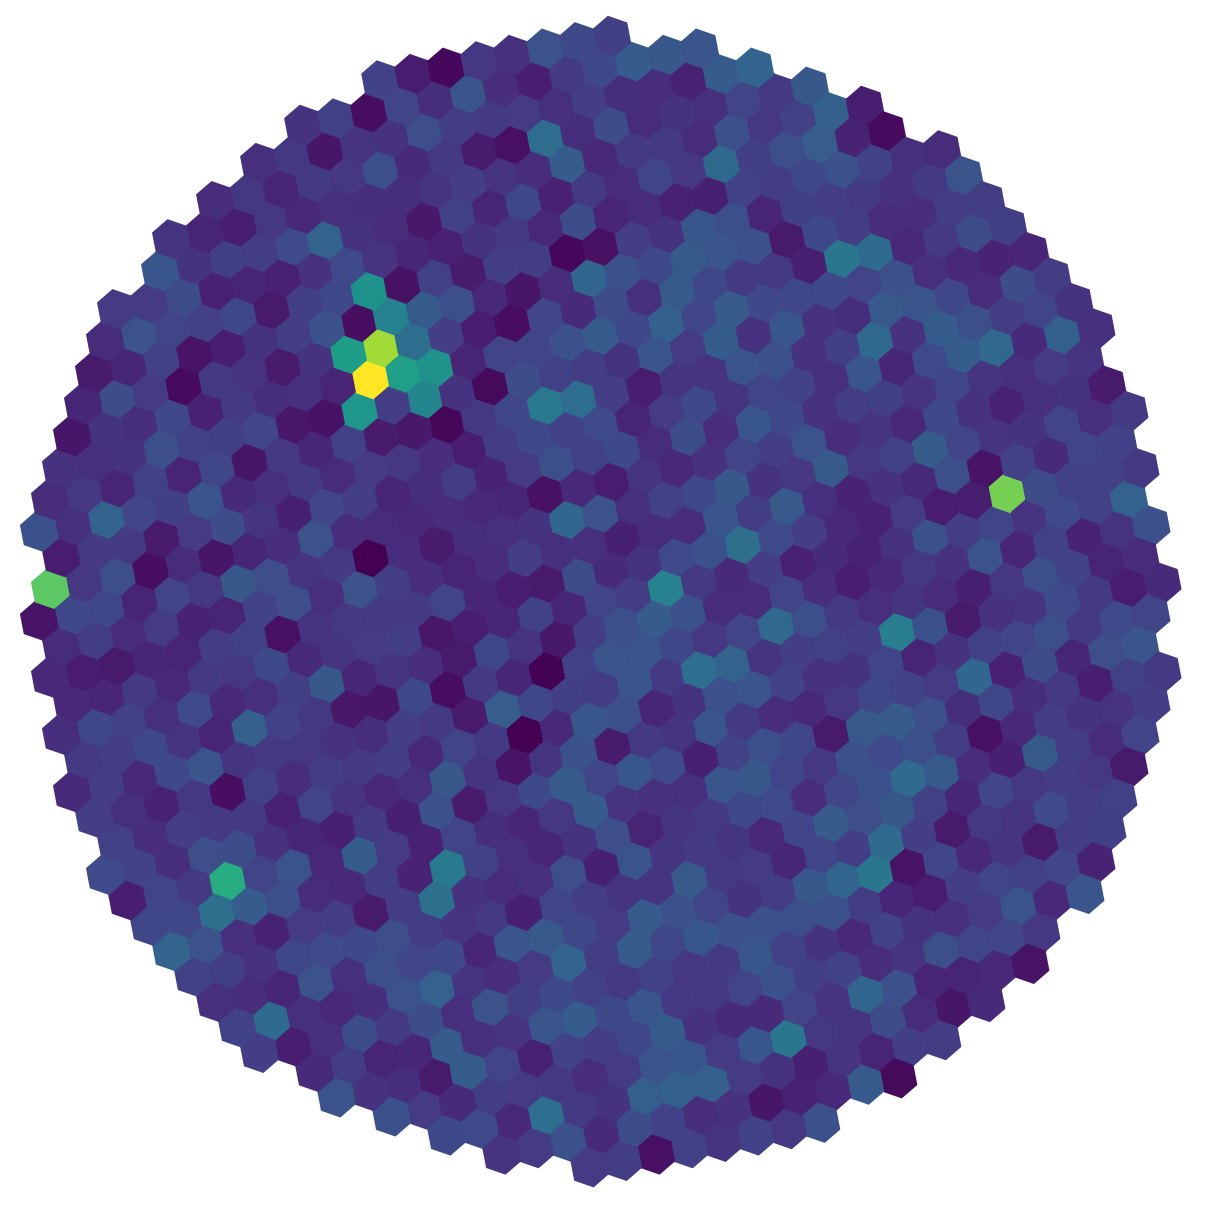
\includegraphics[width=\linewidth]{pictures/uncleaned.png}
    \caption{Kamerabild.}%
    \label{fig:uncleaned}
  \end{subfigure}
  \begin{subfigure}[c]{0.48\linewidth}
    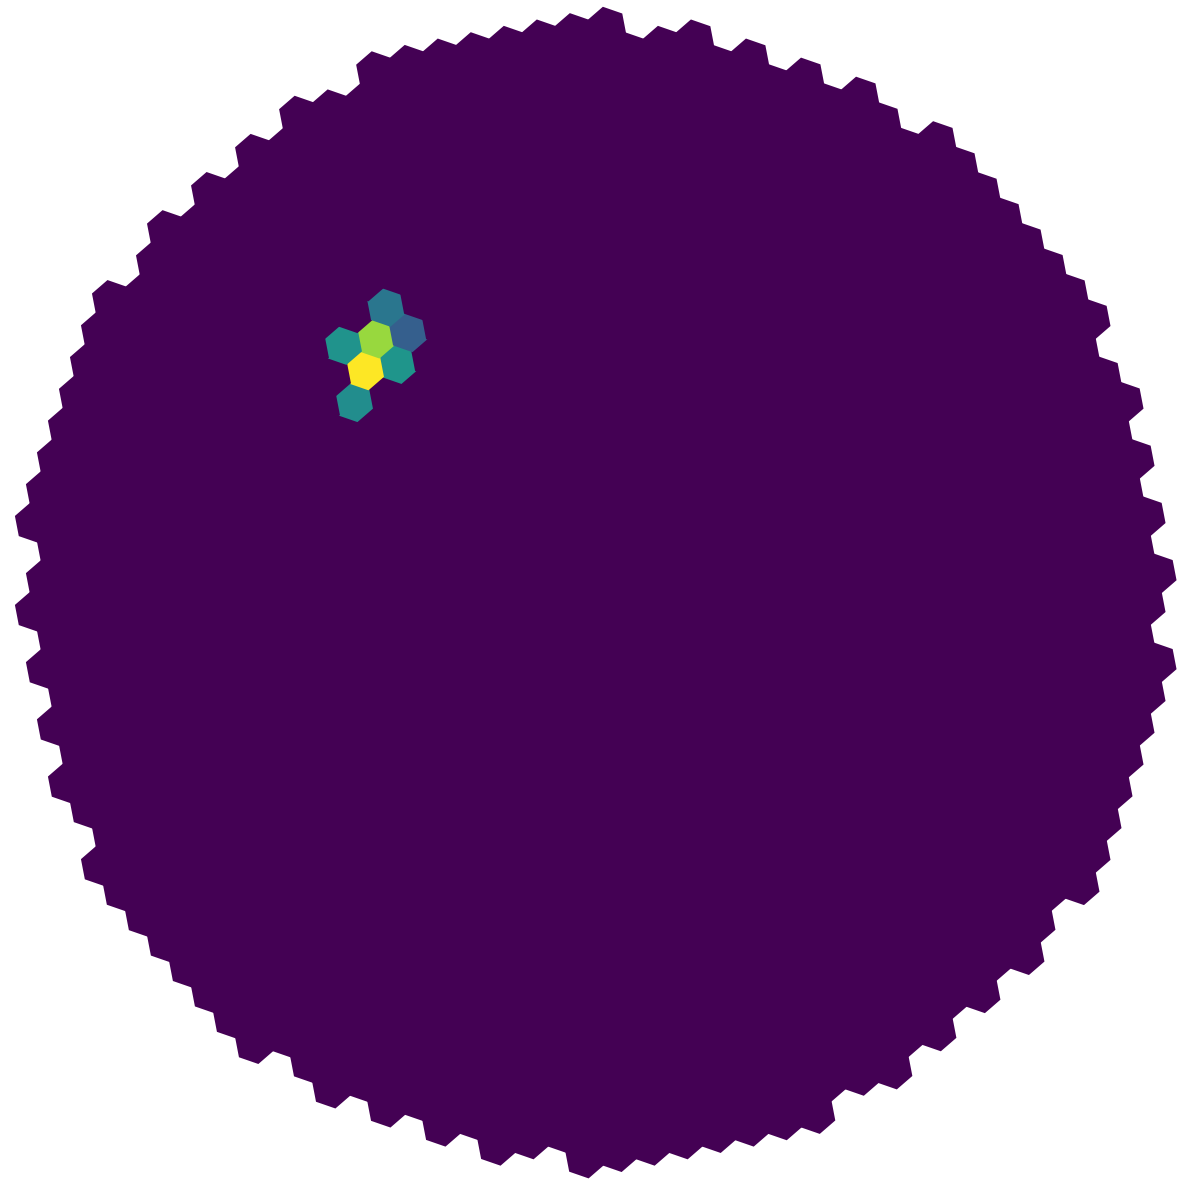
\includegraphics[width=\linewidth]{pictures/cleaned.png}
    \caption{Bereinigtes Kamerabild.}%
    \label{fig:cleaned}
  \end{subfigure}
  \caption{Bereinigung der Kamerabilder zur Berechnung der Hillas Parameter.}%
  \label{fig:cleaning}
\end{figure}

\subparagraph{Hillas Parameter}%
\label{spar:hillas_parameter}

Tscherenkowschauer erzeugen in der Kamera Ellipsenförmige Events.
Anhand der Größe der Ellipse und deren Richtung lässt sich die Energie des
Events bestimmen und die Richtung rekonstruieren.
Dazu wird auf den gereinigten Kamerabildern die Hillas Parameter bestimmt.


\begin{wrapfigure}[15]{o}{0.4\textwidth}
  \centering
  \includegraphics[width=0.8\linewidth]{tikz/build/hillas.pdf}
  \caption{Hillas Parameter eines Schauers.}%
  \label{fig:hillas}
\end{wrapfigure}


Die Hillas Parameter sind width, length, size, con core, disp und theta.
\textit{Width} ist die Nebenachse und \textit{length} die Hauptachse der Ellipse. 
\textit{Size} entspricht der Anzahl an Photonen die im Schauer detektiert wurden.
Da sich der Schwerpunk des Schauers in der Regel nicht mit dem Mittelpunkt der
Ellipse deckt ist dafür der Parameter \textit{Con Core} eingeführt.
Anhand der Parameter \textit{Size} lässt sich der Parameter \textit{dist}
schätzen der die Entferunung des Schauerschwerpunkt zur Rekonstruierten
Quellposition ist.
Die rekonstruierte Quellposition findet sich entsprechend der Orientierung der
Ellipse in einem Abstand von \textit{dist} von dem Schauerschwerpunkt entfernt.
Der Parameter \textit{theta} gibt an wie weit die rekonstruierte von der wahren
Quellposition entfernt ist.
123456789 Satz der noch ersetzt werden sollte damit man schauen kann ob die wrapfigure
richtig funktioniert und schoen aussieht.

\paragraph{Durchführung}
